
% Author: PokMan Ho pok.ho19@imperial.ac.uk
% Script: LogisticTmp.tex
% Desc: Daughter script for corresponding final `LaTeX` report
% Input: none
% Output: none
% Arguments: 0
% Date: Oct 2019

\documentclass[a4paper, 11pt]{article}
\usepackage[margin=1in]{geometry}
\usepackage{hyperref, setspace, lineno}

%% test insert graphs
\usepackage{graphicx}
\graphicspath{ {../results/} } %% <https://www.overleaf.com/learn/latex/Inserting_Images>

%% test insert variables
\newcommand{\ReportTitle}{Report on Logistic Growth curve} %% <https://stackoverflow.com/questions/1211888/is-there-any-way-i-can-define-a-variable-in-latex>
\newcommand{\ReportAuthor}{PokMan HO}
\newcommand{\ReportAffil}{Department of Life Sciences, Faculty of Natural Sciences,\\Imperial College London}
\newcommand{\Disclaim}{\textbf{A Mini-project submitted in partial fulfilment of the requirements for the degree of Master of Research at Imperial College London\\\\Formatted in the journal style of the \textit{Nature} Journal\\Submitted for the MRes in Computational Methods of Ecology and Evolution}}

\title{\ReportTitle}
\author{\ReportAuthor (CID: 01786076)}
\date{}

%% citation
\usepackage[%
autocite    = superscript,
backend     = bibtex,
sortcites   = true,
style       = nature
]{biblatex}
\bibliography{../reference/LogRef.bib} %% <https://tex.stackexchange.com/questions/6805/bib-library-file-in-a-different-directory-how-to-use-mendeley-centralised-b>

%% set as required
\doublespacing
\linenumbers

\begin{document}
	\begin{center}
		\Huge\textbf{\ReportTitle}\\
		\LARGE\ReportAuthor\\
		\Large\ReportAffil
	\end{center}
	\begin{figure}[h]
		\centering
\includegraphics[width=\linewidth]{icl.jpg}
	\end{figure}
	\begin{flushright}
		\Large Approximate Word Count: %% insert approx word count
134
	\end{flushright}
	\clearpage
	
	\maketitle
	\section*{Abstract}
	
	
	\section*{Introduction}
	
	
	\section*{Methods}
	A subset of microbial growth data was selected based on ``the highest number of data points".  The candidate dataset was the replicate %1 %%%%%%% FIRST CUT AFTER THIS %%%%%%%
1
	 from Zwietering \textit{et al.}(1994)\autocite{zwietering1994modeling} \textit{%L.plantarum
Lactobaciulus plantarum
	}on %MRS
MRS
	 substrate under %10
10
	 degrees Celsius.  The data was containing %151
151
	 records on population cell count (%N
N
).\\
	The data was recorded in ``population change" (response variable) against ``time of experiment (hr)" (explanatory variable).  The response variable was neither normally-distributed nor log-normal (Shapiro Test p-value: %0
0
	; Min
0.16
	, 1st Q
3.24
	, 2nd Q
6.55
	, 3rd Q
7.47
	, Max
8.86
	, all corrected to 2 d.p.).  Time (in hr) was also recorded not in a normal-distributed not log-normal way (Shapiro Test p-value: %0
0
	; Min
1.49
	, 1st Q
57.07
	, 2nd Q
123.3
	, 3rd Q
195.36
	, Max
345.07
	, all corrected to 2 d.p.).\\
	modified Gompertz model\autocite{zwietering1994modeling}\\
	Buchanan model\autocite{buchanan1993differentiation}
	\subsection*{Computing tools}
	\section*{Results}
	\begin{figure}[h]
		\centering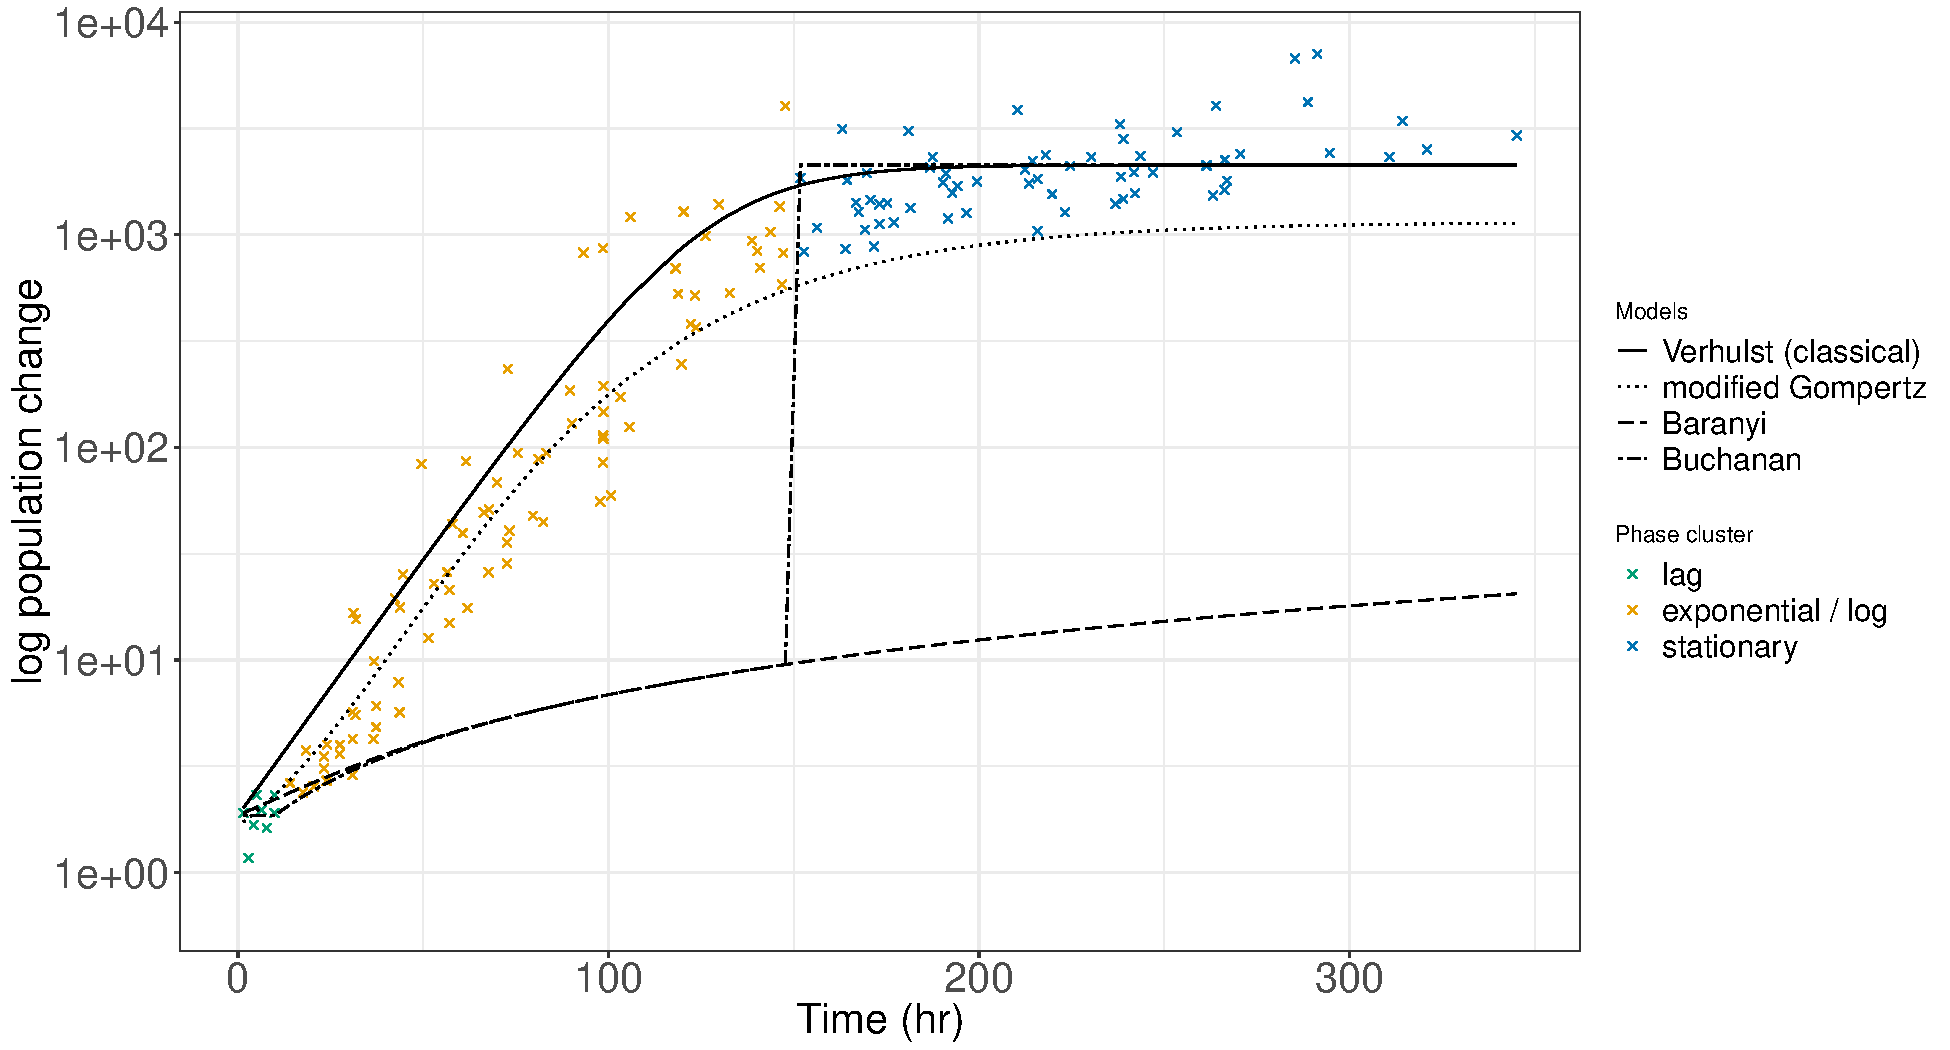
\includegraphics[width=\linewidth]{Log_data.pdf}\label{semi-log}
		\caption{Semi-log graph showing four different models fitting on data of ``Population Change" against ``Experiment time" with points clustered into three main phases of sigmoid growth curve.}
	\end{figure}
	\section*{Discussion}
	\section*{Conclusion}
	\section*{Code and Data Availability}
	All \href{https://github.com/ph-u/CMEECourseWork_pmH/tree/master/MiniProject/code}{scripts} and \href{https://github.com/ph-u/CMEECourseWork_pmH/tree/master/MiniProject/data}{data} used for this report were publicity available at GitHub.
	\nocite{*}\printbibliography
\end{document}